\chapter{Evaluation} % (fold)
\label{cha:evaluation}

Für die Erprobung des Q-Learning-Algorithmuses wurden zwei Linienfolger und eine Teststrecke konzipiert und zusammengebaut. Der Kurs (siehe Abbildung \ref{fig:kurs}) besteht aus verschiedenen Geraden- und Kurvenstücken von variablem Schwierigkeitsgrad.

\begin{figure}[!htb]
	\centering
	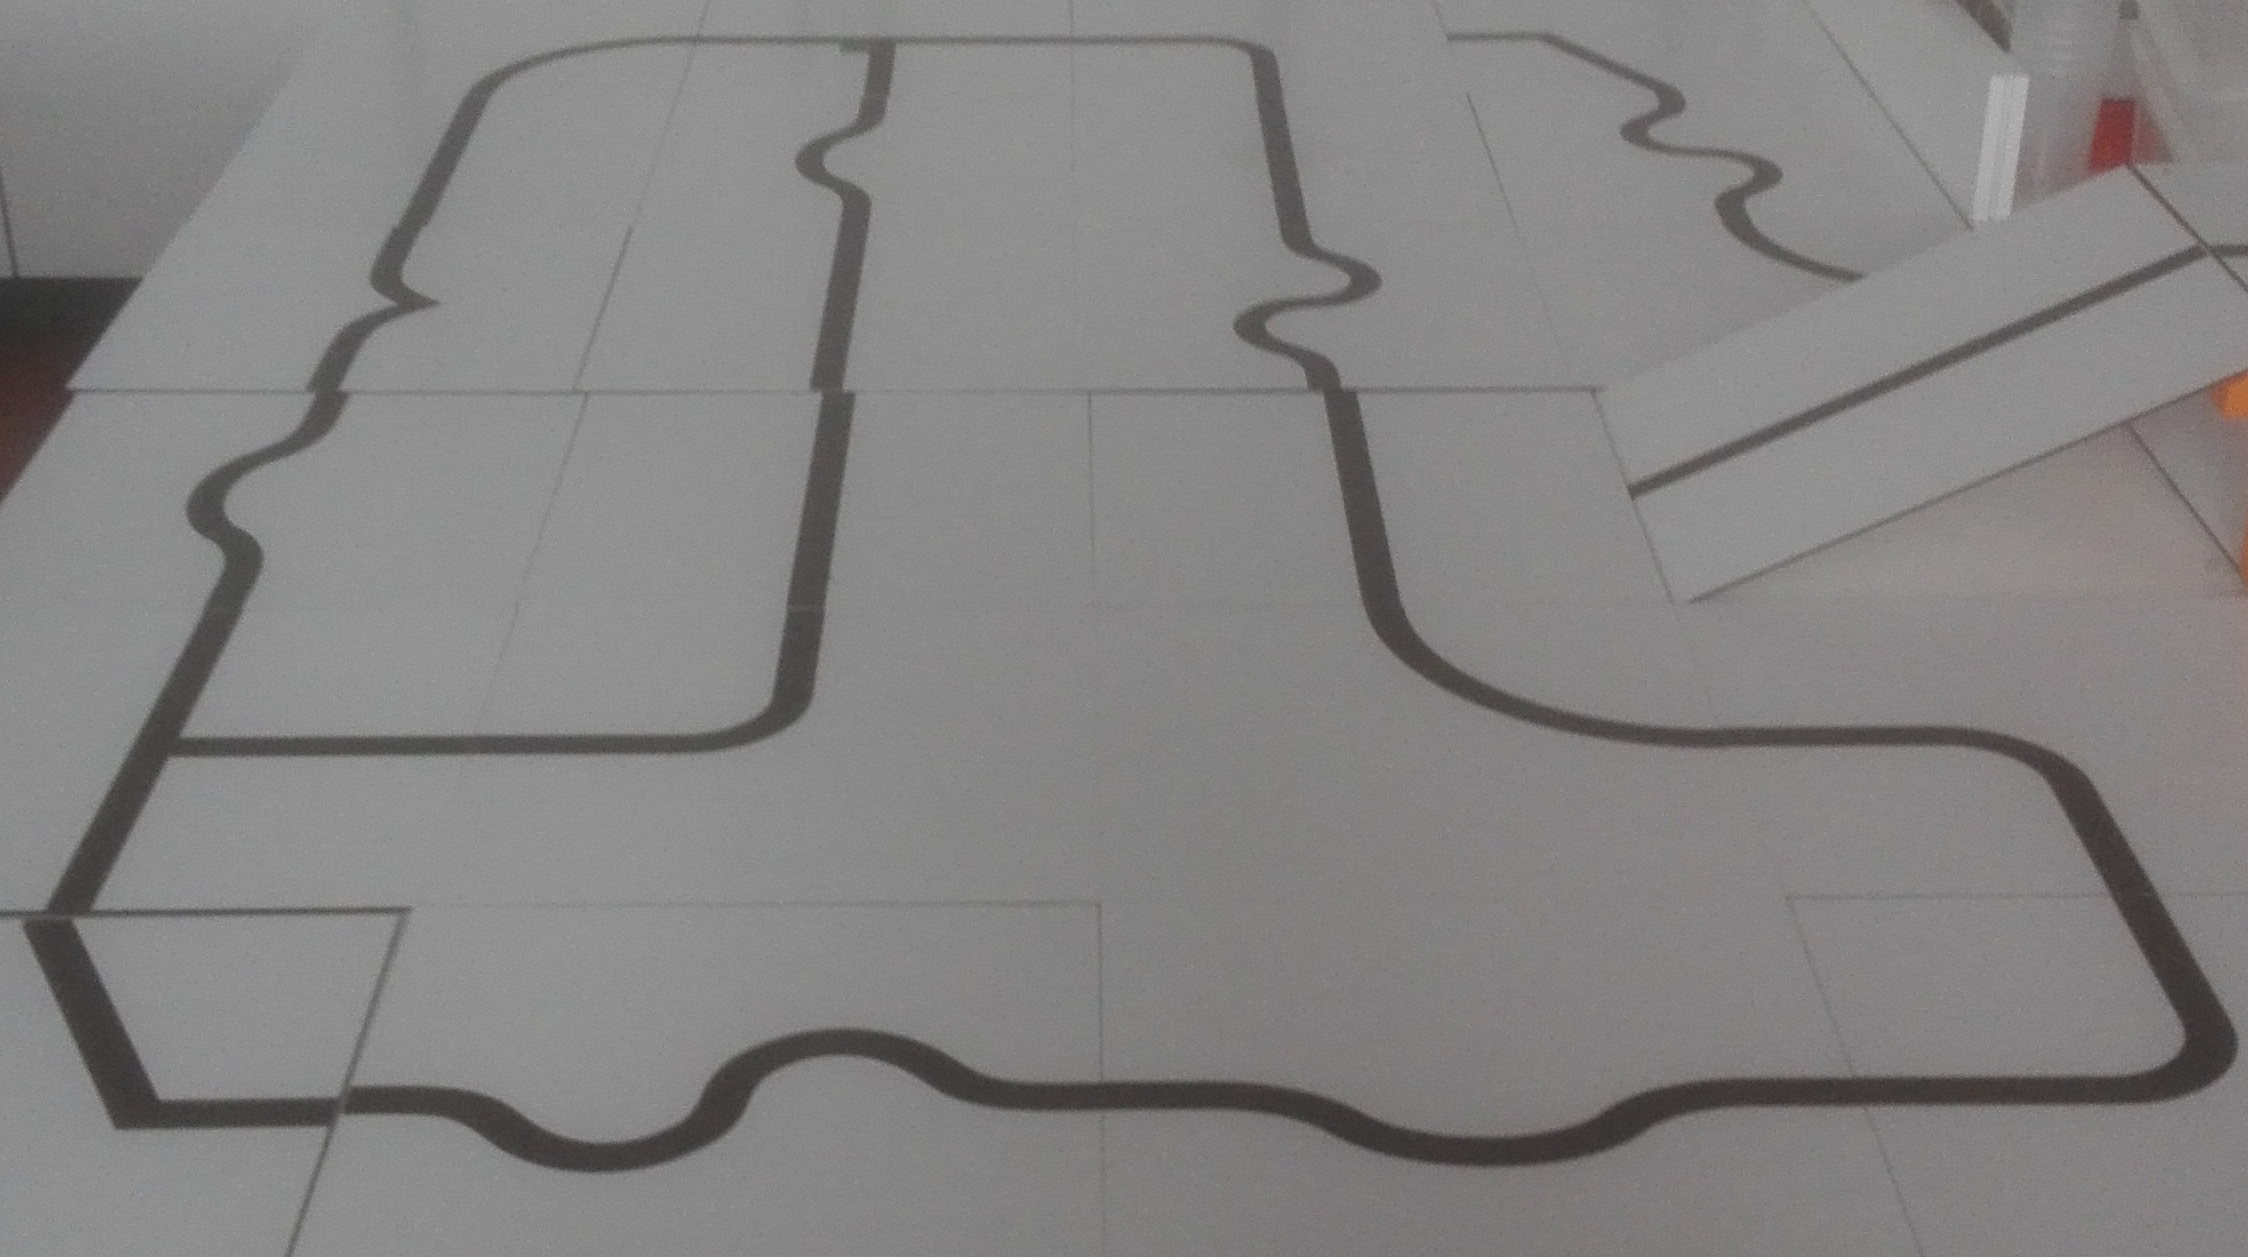
\includegraphics[width=8cm]{kurs.png}
	\caption{Kurs}
	\label{fig:kurs}
\end{figure}

Die beiden Linienfolger unterscheiden sich in der Anzahl und der Anordnung der Farbsensoren. Der erste Linienfolger $L_0$ verfügt über drei Farbsensoren, die nebeneinander angeordnet sind. Die schwarze Linie besitzt dieselbe Breite wie der Lichtkegel eines Farbsensors. Sommit ist der Linienfolger optimal Positioniert falls nur der mittlere Sensor Schwarz und die beiden außenliegenden Sensoren Weiß erkennen. Die Tabelle \ref{tab:zustaende_drei_sensoren} zeigt alle eintretbaren Zustände.

\begin{table}[h]
  \caption{Zustände bei drei Sensoren}
  \label{tab:zustaende_drei_sensoren}
  \renewcommand{\arraystretch}{1.2}
  \centering
  \sffamily
  \begin{footnotesize}
    \begin{tabular}{l l l}
    \toprule
    \textbf{Zustand} & \textbf{Beschreibung} & \textbf{Belohnung}\\
    \midrule
    $s_0$	&	Alle Sensoren erkennen Weiß.	&	0\\ % 000
    $s_1$	&	Der rechte Sensor erkennt Schwarz.	&	0\\ % 001
    $s_2$	&	Der mittlere Sensor erkennt Schwarz.	&	0\\ % 010
    $s_3$	&	Der mittlere und rechte Sensor erkennt Schwarz.	&	0\\ % 011
    $s_4$	&	Der linke Sensor erkennt Schwarz.	&	0\\ % 100
    $s_5$	&	Der linke und rechte Sensor erkennt Schwarz.	&	0\\ % 101
    $s_6$	&	Der linke und mittlere Sensor erkennt Schwarz.	&	0\\ % 110
    $s_7$	&	Alle Sensoren erkennen Schwarz.	&	0\\ % 111
    \bottomrule
    \end{tabular}
  \end{footnotesize}
  \rmfamily
\end{table}

Im Gegensatz zum ersten Linienfolger besitzt der zweite Linienfolger $L_1$ zwei Farbsensoren, die angewinkelt angeordnet sind. Sommit besitzt er andere Zustände als $L_0$, diese sind in der Tabelle \ref{tab:zustaende_zwei_sensoren} beschrieben.

\begin{table}[h]
  \caption{Zustände bei zwei Sensoren}
  \label{tab:zustaende_zwei_sensoren}
  \renewcommand{\arraystretch}{1.2}
  \centering
  \sffamily
  \begin{footnotesize}
    \begin{tabular}{l l l}
    \toprule
    \textbf{Zustand} & \textbf{Beschreibung} & \textbf{Belohnung}\\
    \midrule
    $s_0$	&	Beide Sensoren erkennen Weiß.	&	0\\
    $s_1$	&	Der rechte Sensor erkennt Schwarz.	&	0\\
    $s_2$	&	Der linke Sensor erkennt Schwarz.	&	0\\
    $s_3$	&	Beide Sensoren erkennen Schwarz.	&	1\\
    \bottomrule
    \end{tabular}
  \end{footnotesize}
  \rmfamily
\end{table}

Zur Erreichung eines anderen Zustandes können beide Linienfolger folgende Aktionen (siehe Tabelle \ref{tab:aktionen}) ausführen. Die Art der Ausführung unterscheidet sich nicht bei $L_0$ oder $L_1$.

\begin{table}[h]
  \caption{Aktionen}
  \label{tab:aktionen}
  \renewcommand{\arraystretch}{1.2}
  \centering
  \sffamily
  \begin{footnotesize}
    \begin{tabular}{l l}
    \toprule
    \textbf{Aktion} & \textbf{Beschreibung}\\
    \midrule
    $a_0$	&	Linkskurve\\
    $a_1$	&	Ge­ra­de­aus­fahrt\\
    $a_2$	&	Rechtskurve\\
    \bottomrule
    \end{tabular}
  \end{footnotesize}
  \rmfamily
\end{table}

Beide Linienfolger nutzen für das Q-Learning die gleichen Parameter, um die Vergleichbarkeit der Ergebnisse zu gewährleisten.

\begin{table}[h]
  \caption{Q-Learning-Parameter}
  \label{tab:q-parameter}
  \renewcommand{\arraystretch}{1.2}
  \centering
  \sffamily
  \begin{footnotesize}
    \begin{tabular}{l l}
    \toprule
    \textbf{Parameter} & \textbf{Wert}\\
    \midrule
    $\alpha$	&	$0.9$\\
    $\gamma$	&	$0.2$\\
    $\epsilon$	&	$0.01$\\
    \bottomrule
    \end{tabular}
  \end{footnotesize}
  \rmfamily
\end{table}

Die optimale Strategie für $L_0$ ist im Graph \ref{fig:zwei_sensoren_optimale_strategie} angegeben, die für $L_1$ in Graph \ref{fig:drei_sensoren_optimale_strategie}.

\begin{figure}
\centering
\begin{tikzpicture}[->,>=stealth',shorten >=1pt,auto,node distance=3cm,
                    thick,main node/.style={circle,draw,font=\sffamily\Large\bfseries}]

  \node[main node] (1) {$s_1$};
  \node[main node] (2) [below left of=1] {$s_0$};
  \node[main node] (3) [below right of=2] {$s_3$};
  \node[main node] (4) [below right of=1] {$s_2$};

  \path[every node/.style={font=\sffamily\small}]
    (1) edge node [left] {$a_0$} (3)
    (2) edge node [left] {$a_0$, $a_1$, $a_2$} (3)
    (3) edge [loop below] node {$a_1$} (3)
    (4) edge node [left] {$a_2$} (3);
\end{tikzpicture}
\caption{Optimale Strategie bei zwei Sensoren} 
\label{fig:zwei_sensoren_optimale_strategie}
\end{figure}

\begin{figure}
\centering
\begin{tikzpicture}[->,>=stealth',shorten >=1pt,auto,node distance=3cm,
                    thick,main node/.style={circle,draw,font=\sffamily\Large\bfseries}]

  \node[main node] (1) {$s_2$};
  \node[main node] (2) [below left of=1] {$s_1$};
  \node[main node] (3) [below right of=1] {$s_3$};
  \node[main node] (4) [below left of=2] {$s_0$};
  \node[main node] (5) [below right of=3] {$s_4$};
  \node[main node] (6) [below right of=4] {$s_7$};
  \node[main node] (7) [below left of=5] {$s_5$};
  \node[main node] (8) [below right of=6] {$s_6$};


  \path[every node/.style={font=\sffamily\small}]
    % (1) edge node [left] {$a_1$} (4)
    %     edge [bend right] node[left] {0.3} (2)
    %     edge [loop above] node {0.1} (1)
    % (2) edge node [right] {0.4} (1)
    %     edge node {0.3} (4)
    %     edge [loop left] node {0.4} (2)
    %     edge [bend right] node[left] {0.1} (3)
    % (3) edge node [right] {0.8} (2)
    %     edge [bend right] node[right] {0.2} (4)
    % (4) edge node [left] {0.2} (3)
    %     edge [loop right] node {0.6} (4)
    %     edge [bend right] node[right] {0.2} (1);
    (1) edge [loop left] node {$a_1$} (1)
    (2) edge node [above] {$a_2$} (3)
    (3) edge node [right] {$a_2$} (1)
    (4) edge node [left] {$a_2$} (2)
    	edge [bend above] node[above] {$a_0$} (5)
    (5) edge [bend left] node {$a_0$} (8)
    (6) edge node [left] {$a_0$} (8)
    	edge node [right] {$a_2$} (3)
    (7) edge node [left] {$a_0$} (5)
    	edge node [left] {$a_2$} (2)
    (8) edge [bend left] node[left] {$a_0$} (1);
\end{tikzpicture}
\caption{Optimale Strategie bei drei Sensoren} 
\label{fig:drei_sensoren_optimale_strategie}
\end{figure}

Bei beiden Linienfolgern wurden die optimalen Aktionen für alle Zustände alle 50 Lernschritte protokoliert.

% chapter evaluation (end)